
%%%%%%%%%%%%%%%%%%%%%%%%%%%%%%%%
\section{Propulsion Power Modeling, Estimation, Runtime Optimization, and Design-Time Optimization} \label{sec:propulsion}
%%%%%%%%%%%%%%%%%%%%%%%%%%%%%%%%

Electric vehicles of course consume majority of electrical energy for propulsion. Electric vehicle propulsion energy generally increases proportionally to their weight but also largely variable by the driving conditions such as road slope. Unfortunately, electric vehicles are not lighter than the similar scale of internal combustion engine vehicles due to the battery weight while production electric vehicles deploy light materials such as aluminum to a large portion of chassis and bodies to compensate the battery weight. For instance, Chevrolet Bolt (164” long) weighs 3563 lbs, but a Honda Civic (177” long) does only 2752 lbs.

Electric powertrain efficiency is already close to the their theoretical limits. Electric vehicles also have advantages in well-to-wheel efficiency from idling, downhill driving and braking using regenerative braking. Nevertheless, the well-to-wheel efficiency of electric vehicles is not much higher than that of internal combustion engine vehicles. Regenerative braking is fundamental advantage of electric vehicles that reclaim kinetic energy back to electrical energy, which is dissipated to heat energy in the internal combustion engine vehicles. However, modern internal combustion engine vehicles adopt engine stop-and-go during idle and also regenerative braking using the alternator.

%%%%%%%%%%%%%%%%%%%%%%%%%%%%%%%%
\subsection{Propulsion Power Modeling} \label{subsec:propulsion_model}

% Come from section {sec:driving_profile}
Electric Vehicle as a multi-domain Cyber-Physical System (CPS) consists of two major systems of electric motor and auxiliary system that are the main contributors to the power consumption~\cite{AF_1,AF_2,AF_3,Park:DAC13}.

\textbf{Electric motors} are the key components of the propulsion system that generates force to propel the vehicle at a desired speed and acceleration. The electric motor consumes battery energy to produce driving force but can also behave as a generator when the applied torque becomes negative during deceleration. This regenerative braking system helps the electric vehicles achieve higher energy efficiency and extended driving range~\cite{AF_5,AF_6,AF_7}.

\textbf{Propulsion power} generated or consumed by the electric motor significantly influences the stored battery energy, the electric vehicle driving range, and the battery lifetime~\cite{AF_8,AF_9,AF_10}. Hence, modeling, estimation, and optimization of the propulsion power are mandatory tools and methodologies to extend the driving range and battery lifetime.

\subsubsection{Physics Model} \label{subsubsec:physical_model}

Most of all, accurate propulsion power modeling is the basis of electric vehicle power estimation, runtime power management and design-time power optimization. Vehicle propulsion power modeling has been used for eco-driving research for internal combustion engine vehicles over decades. An underlying propulsion power model is based on well-known physics equations. Such vehicle dynamics model basically takes into account the propulsion power applied to the tires.

\begin{equation} \label{eq:traction_model}
P_{trac} = F \frac{ds}{dt} = Fv= (F_{R} + F_{A} + F_{G} + F_{I} + F_{B}) v
\end{equation}
%
where $F_R$, $F_A$, $F_G$, $F_I$, and $F_B$ are the rolling resistance, aerodynamic resistance, gradient resistance, inertia resistance, and brake force provided by hydraulic brakes, respectively~\cite{Chang:ICCAD14, Park:DAC13}. This model applies to all type of propulsion systems as it assumes 100\% efficiency of the propulsion system. As a result, this physics model does not explain electric-vehicle-specific power consumption behaviors such as electric traction motor characteristics, regenerative braking, battery efficiency, etc. Such simplification still can marginally estimate electric vehicle propulsion power but hardly use for propulsion power saving research.

One need to obtain the actual model coefficients for actual deployment of the power models of~\eqref{eq:traction_model}. Vehicle manufacturers often provide a part of model coefficients in the specification sheet such as the aerodynamic resistance as well as the curb weight, and tire manufactures commonly advertises the rolling resistance values of their products. Wind chamber experiments can also obtain unknown aerodynamic resistance values.

\subsubsection{Motor Efficiency} \label{subsubsec:motor_eff}

The primary discrepancy between the electric vehicles and internal combustion engine vehicles can be explained by the source of the propulsion power: electric motors and internal combustion engines. Adding the electric motor characteristics to the physics model in~\eqref{eq:traction_model} is able to accommodate electric powertrain characteristics.

\begin{figure}
\centering
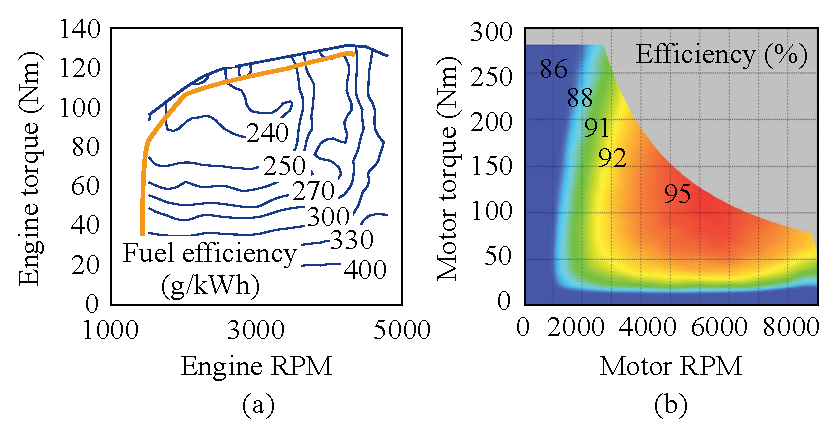
\includegraphics[width=1.0\hsize]{Figures/Naehyuck_Chang/motor_engine_torque_map.pdf}
\caption{A 1.4 liter GM Voltec Internal combustion engine efficiency map (a) and a Nissan Leaf 80kW electric motor efficiency map (b)~\cite{Nissan:SAE11, Grebe:ATZ11}.}
\label{fig:torque_map}
\end{figure}      

Fig.~\ref{fig:torque_map}(a) illustrates efficiency maps of a 1.4 liter GM Voltec engine and a Nissan Leaf 80kW motor. Electric vehicle efficiency is largely different from that of engine vehicles even under the same driving condition as the source of the traction force is a completely different characteristics, even if electric vehicles are subject to~\eqref{eq:traction_model} as well. Electric motor efficiency varies by the motor type, motor revolution per minute (RPM) and torque. Consideration of traction device efficiency can significantly enhance the electric-vehicle-specific characteristics over~\eqref{eq:traction_model} as shown as

\begin{align} \label{eq:motor_eff_model}
P_{EV} &= \frac{P_{trac}}{\eta_{EV}} \\
\eta_{EV} &= \frac{P_{trac}}{{P_{trac} + k_c T^2 + k_i \omega + k_w \omega^3 + C}}, \nonumber
\end{align}
%
where $k_c$, $k_i$, $k_w$, $C$ are a copper loss, a iron and friction loss, a windage loss and constant loss, respectively~\cite{Vaz:JPS14,Lin:CCA14,Oliva:PHM13,Kachroudi:TVT12}.

\subsubsection{Drivetrain Efficiency} \label{subsubsec:drive_eff}

Power consumption model in of~\eqref{eq:motor_eff_model} reflects efficiency of the electric motors. The actual electric vehicle propulsion efficiency is not only dependent on the traction motor but affected by the drivetrain loss in the gearbox, axle bearings, driveshaft, gearbox fluid, and many more, which varies by the vehicle speed, acceleration and motor torque. The actual model coefficients can be obtained from the motor companies, but this is not always the case.
It is hard to rely on vehicle specification sheets to figure out drivetrain efficiency. Test run in various conditions helps collect range of power consumption data and obtain the model coefficients by a curve fitting method~\cite{Dib:OGST12} with a high model fidelity of 1.7\% overall cumulative energy consumption error~\cite{Dib:OGST12}. A dynamometer test provides an isolated experimental environment~\cite{Schwickart:JFI15} to obtain the actual efficiency of the traction motor combined with the drivetrain.

Consideration of accurate efficiency change of the traction motors and drivetrain loss can be highly nonlinear, and thus it is challenging to use mathematical equation models such as~\eqref{eq:traction_model} and~\eqref{eq:motor_eff_model}. Lookup tables are convenient to describe complicated power characteristics and also easy to implement a power simulator~\cite{Schwickart:JFI15} while less convenient to use for systematic optimization.

More precise electric vehicle power modeling requires extensive power measurement and characterization. Use of production electric vehicles brings various limitations in non-intrusive power measurement. Fabrication of an electric vehicle~\cite{Hong:ASPDAC16} or electric vehicle conversion of a production internal combustion engine vehicle~\cite{Wu:TR15} efficiently overcomes the limitation in non-intrusive power measurement. The battery power should be measured together with the vehicle driving condition. Global positioning system (GPS) provides the location, altitude and thus road slopes. Such whitebox experiments efficiently isolate the propulsion power consumption from non-propulsion power consumption and give a lot of benefits in power modeling~\cite{Hong:ASPDAC16,Wu:TR15}. It turns out that drivetrain loss in the electric vehicle is proportional to the square of the vehicle speed while the electric powertrain model only has a linear term of the speed as shown in~\eqref{eq:drive_eff_model}~\cite{Hong:ASPDAC16}.

\begin{align} \label{eq:drive_eff_model}
P_{EV-specific} &= \frac{P_{trac}}{\eta_{EV-specific}} \\
\eta_{EV-specific} &= \frac{P_{trac}}{{P_{trac} + C_0 + C_1 v + C_2 v^2 + C_3 T^2}} \nonumber
\end{align}
%
where $C_0$, $C_1$, $C_2$, and $C_3$ mean coefficients for constant loss, iron and friction
losses, drivetrain loss, and copper loss, respectively. These methods guarantee a very high estimation accuracy (e.g., 2.89\% maximum absolute error in~\cite{Hong:ASPDAC16}) for the target vehicle model. However, these models ensure limited accuracy when applied to general electric vehicles.

\subsubsection{Electric Vehicle Driving Range Estimation} \label{subsubsec:range_est}

Most electric vehicle owners have range anxiety due to the limited driving range as well as inaccurate remaining range gauge on the instrument cluster. Depletion of the vehicle battery in the middle of a trip may bring a trouble equivalent to vehicle breakdown~\cite{Hong:ASPDAC16}.

The electric vehicle power models of~\eqref{eq:traction_model}-\eqref{eq:drive_eff_model} require vehicle weight, acceleration, speed, and road slope as the input variables. It is impossible to know the actual values of the future vehicle acceleration and speed in real cases due to the uncertainty in the driving conditions. Such unknown factors can be modeled as probability density functions, and the resultant driving range estimation can also be represented probabilistically. This work models the uncertainty with a statistical speed profile~\cite{Oliva:PHM13}.

Consideration of the battery characteristics is also attempted such as the state of charge versus the battery output voltage. For example, battery current keeps increasing as battery discharges even if the vehicle maintain a constant cruising speed on a flat road~\cite{Vaz:JPS14}. This work assumes that the vehicle speed should be decreased as the battery voltage decreases, but which is not in the real case because the battery should be cut off before it becomes fully discharged (over-discharge protection typically at 20\% SoC) by the battery management system (BMS), and the motor driver should be able to maintain the same torque within the legal voltage range of the battery.

The fidelity of the power consumption model directly impacts on the range estimation accuracy~\cite{Hong:ASPDAC16}. The power model in~\eqref{eq:drive_eff_model} that considers the drivetrain efficiency exhibits less than 2.89\% maximum absolute error in the power consumption, and thus between 0.05\% to 4.39\% in range estimation compared with real measurement~\cite{Hong:ASPDAC16}. On the other hand, the power models in~\eqref{eq:traction_model} and~\eqref{eq:motor_eff_model}, which consider only propulsion power and motor efficiency, obtain 6.85\% and 9.33\% maximum absolute error in the power consumption and up to 19.19\% and 21.75\% in range estimation, respectively.

%%%%%%%%%%%%%%%%%%%%%%%%%%%%%%%%
\subsection{Runtime Propulsion Power Optimization} \label{subsec:propulsion_runtime_opt}

A large portion of previous work relies on the physics model in~\eqref{eq:traction_model} or adding the motor efficiency in~\eqref{eq:motor_eff_model} to estimate electric vehicle power consumption. Therefore, derivation of the energy-optimal vehicle speed for a given road slope is often attempted with~\eqref{eq:traction_model} or~\eqref{eq:motor_eff_model}~\cite{Wu:TR15,Vaz:JPS14,Lin:CCA14,Oliva:PHM13,Kachroudi:TVT12}.
As mentioned in Section I, electric vehicles consume different amount of power and energy by the vehicle speed and acceleration due to the non-constant efficiency of the traction motor and the drivetrain even if the vehicles drive on the same route with the same payload. This inspires runtime propulsion power optimization, which is a similar concept of eco-driving of internal combustion engine vehicles~\cite{Kamal:TITS11,Ozatay:IFAC14,Ozatay:TITS14,Khayyam:ESA12}. However, the fundamental discrepancy in the electric powertrain from the engine powertrain makes the optimization policy largely different.

\subsubsection{Propulsion Power Optimization with a Constant Road Slope} \label{subsubsec:opt_const_slope}

According to the electric vehicle power model in~\eqref{eq:drive_eff_model}, propulsion power varies by the road slope as well as the vehicle speed, and thus the total energy consumption to finish the same distance of travel, i.e., the integration of the vehicle power over the driving time, forms a convex function of the vehicle speed for a given constant road slope as shown in Fig.~\ref{fig:energy_vs_vel}. The shape of the convex function varies by the road slope, which implies that there exists the energy-optimal electric vehicle speed by a given road slope.

\begin{figure}
\centering
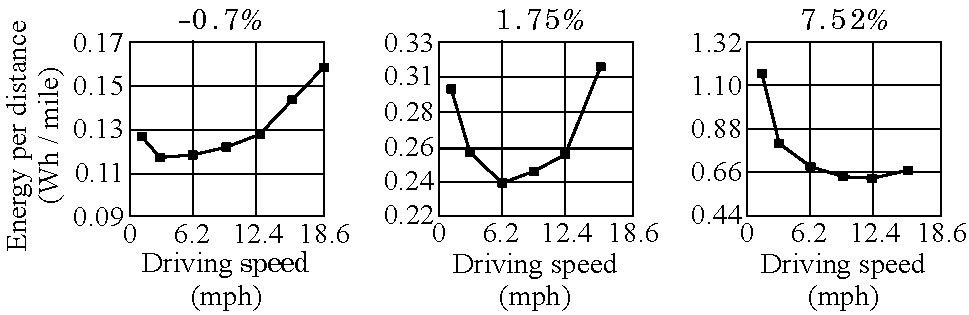
\includegraphics[width=1.0\hsize]{Figures/Naehyuck_Chang/energy_consumption_by_velocity.pdf}
\caption{Energy consumption versus electric vehicle speed on various road slopes.}
\label{fig:energy_vs_vel}
\end{figure}      

It is very interesting to note that the energy-optimal speed increases by the road slope in the case of electric vehicles, i.e., electric vehicles should run faster on a steeper road to save energy. This inspires the minimum-energy speed planning over time (or distance) for a given driving mission: a route, a payload and a deadline, which is electric-vehicle-specific. Therefore, one of the simplest propulsion power optimization problem is defined as finding the energy-optimal vehicle speed planning (acceleration, cruising and deceleration) for a given constant road slope.
Related previous work derives the energy-optimal vehicle speed planning without considering the traffic condition assuming a constant road slope~\cite{Yan:NAPS14,Dib:CEP14}. A trapezoidal driving, a combination of a constant acceleration, a constant speed cruising and a constant deceleration, is not an impractical driving method even in the real world with a smooth traffic flow, and a series of trapezoidal driving patten planning accommodates intersections with stop signs~\cite{Yan:NAPS14}. Fast computation is always beneficial for practical use to eventually accommodate traffic condition and route change guided by GPS navigation systems. A simplified analytical method that ignores aerodynamic resistance and motor efficiency help rapidly solve the energy-aware trapezoidal driving problem~\cite{Dib:CEP14}.

\subsubsection{Propulsion Power Optimization with a Variable Road Slope} \label{subsubsec:opt_variable_slope}

Many cities are located on hills as well as on flat lands. The energy-optimal trapezoidal driving may not work if the road slope varies before a single trapezoidal driving ends. The trapezoidal driving with a constant cruising speed is no longer energy optimal if the road slope changes. Consideration of the road slope change is crucial for freeway driving where there is no traffic signal nor intersection with stop signs.

The problem to solve the propulsion power optimization with a variable road slope is formulated as an optimal speed selection problem over distance as shown in Fig.~\ref{fig:formulation}(a). The X-axis and Y-axis in Fig.~\ref{fig:formulation}(b) denote the driving distance from the starting point and the driving speed, respectively. Each node indicates the driving speed at a given distance, and an edge between two nodes implies acceleration or deceleration during the distance step.

\begin{figure}
\centering
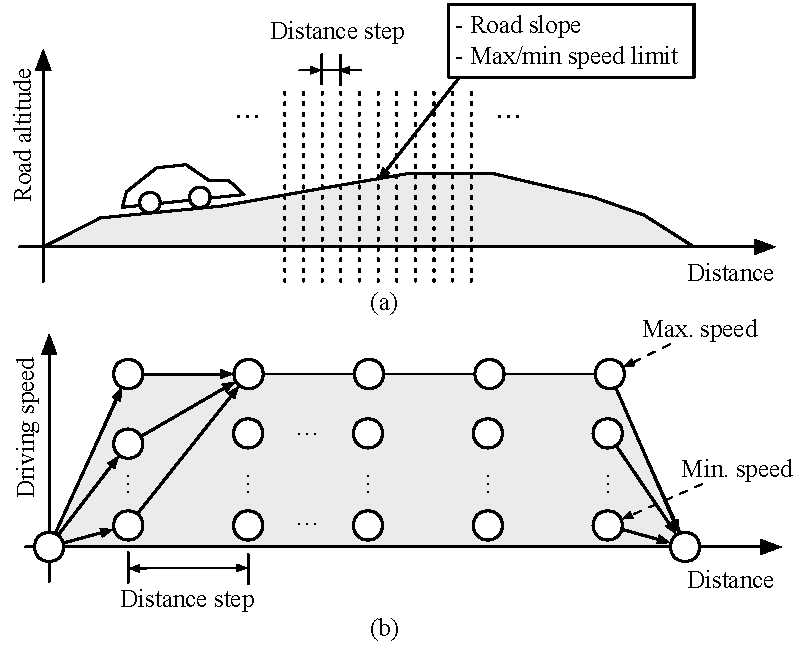
\includegraphics[width=1.0\hsize]{Figures/Naehyuck_Chang/Discretization.pdf}
\caption{Problem formulation for the propulsion power optimization with a variable road slope.}
\label{fig:formulation}
\end{figure}      

The energy-optimal speed profiles exhibit dynamically changing cruising speed taking the regenerative braking and speed limit into consideration as well. Previous work tackles this problem without considering the traffic condition and stop signs by the use of analytical method~\cite{Kamal:TITS11,Ozatay:IFAC14}, dynamic programming~\cite{Ozatay:TITS14}, machine learning~\cite{Khayyam:ESA12}, and model predictive control~\cite{Schwickart:JFI15}. Model predictive control (MPC) derives the optimal motor torque with the objective of a weighted sum of the energy consumption in every 400 m drive and the kinetic energy difference between the best constant speed and the derived speed~\cite{Schwickart:JFI15}. These methods derives the energy-optimal speed profiles on a variable-slope road with a reasonable computational complexity but can hardly guarantee the deadline constraint.

Even if dynamic programming can hardly guarantee a hard deadline while minimizing the driving energy, making the cost function as a weighted average of the driving time and driving energy is able to consider the deadline in a certain degree~\cite{Dib:IVPPC11,Dib:OGST12,Mensing:TR13,Lin:CCA14}. This method is useful for soft real-time system, which is the case of most common driving missions.

The dynamic programming with an weighting factor is formulated with follow:

\begin{align} \label{eq:dynamic_programming}
min ~& \sum_{d=1}^{M}\sum_{v=1}^{N}\{w \Delta t x(d,v)P_{d,v} + (1-w)\Delta t \}\\
Subject~to ~& \sum_{v=1}^{N}x(d,v) = 1~~~\forall v \nonumber \\
~&x(d,v) = \{0, 1\} ~~~\forall d, v \nonumber
\end{align}
%
where $\Delta t$ is a driving time during the distance step, $d$ is a distance from the start point, $v$ is a speed at the distance, $P_{d,v}$ is a power consumption at a distance $d$ and a speed $v$, and w is weighting factor. $\Delta t$ is varied by the driving speed and the acceleration during the distance step.

A more explicit deadline awareness can be derived by iterative methods or semi-exhaustive heuristics that forms a multi-objective optimization problem such as genetic algorithm~\cite{Kachroudi:TVT12,Dovgana:ASC14}. However, these methods are subject to a very high computational complexity, which can be hardly used for online methods that are reactive to the traffic condition change and unexpected interruption by other cars or pedestrians.

\subsubsection{Propulsion Power Optimization Considering Traffic and Intersections} \label{subsubsec:opt_traffic}

The energy-optimal driving method introduced in the previous sections may not actually feasible in real traffic conditions. Safety is always first than energy saving, and thus heavy traffic often makes the vehicle slow down than the energy-optimal speed. Such traffic condition cannot be fully known a priori, and the derived energy-optimal driving method should be computed again whenever unexpected disturbance happens, which ends up with a local minimum energy consumption. Consideration of the traffic condition and traffic signal makes the energy-optimal driving more realistic~\cite{Mensing:TR13,Lim:TVT17,Mandava:ITSC09,Asadi:TCST11,Ozatay:CDC13,Nunzio:JRNC15,Wu:ITS15}  even if such work is still based on strong assumptions. Such work is rather a high-level driving problem rather than electric vehicle-specific driving energy optimization.

Average speed of preceding vehicles on the same route marginally explains the distance between vehicles, which constrains the maximum possible target vehicle speed~\cite{Mensing:TR13,Lim:TVT17}. Traffic signals are often controlled by a periodic schedule that mimics the energy-optimal driving~\cite{Mandava:ITSC09,Asadi:TCST11,Ozatay:CDC13,Nunzio:JRNC15,Wu:ITS15}.

A majority portion of intersection driving management is to optimize the throughput. There are intersection driving management work that explicitly optimize driving energy~\cite{Nunzio:JRNC15,Wu:ITS15} demonstrating 8\% to 48\% energy saving. Once again, such work does not perform electric-vehicle-specific driving energy optimization, and consideration of electric powertrain and regenerative braking may exhibit a large difference in the energy consumption.
\textcolor{red}{
\subsubsection{Propulsion Power Optimization minimizing EV life-cycle cost:} \label{subsubsec:opt_life_cycle}
A cycle life of an EV battery is largely limited by its chemistry, but the charge/discharge behavior also significantly affects the cycle life \cite{Battery SoH model due to DOD - can Sarre:JPS04 be used here too?}. From the EV owners' perspective, the total cost of ownership that includes the EV cost (battery chemistry and capacity -- design-time optimization), electricity usage (runtime power management) and battery aging (residual value and/or replacement cost) are equally important. The total cost of ownership optimization for a dedicated user is a very complicated problem and yet is an open problem. 
%The propulsion power optimization minimizing EV life-cycle cost is very important problem for owners since the battery aging varies depending on the speed planning, and directly linked to cost of maintenance increases.
%It is very complex to solve the optimization problem because we should consider the battery aging mechanism and road information as well as EV powertrain at the same time.\\
%
However, there have been several research practices on battery aging and guidelines to extend the EV battery cycle life~\cite{Sarre:JPS04,Keil:PHD17}. Related work performed experiments to analyze the battery performance (capacity and allowable peak power) by cycle times under various driving conditions (\textit{e.g.}, the temperature, driving profiles, etc.) Such work proposeds guidelines under both non-operating condition and operating condition based on the experimental results.}
%%%%%%%%%%%%%%%%%%%%%%%%%%%%%%%%
\subsection{Design-Time Propulsion Power Optimization} \label{subsec:propulsion_design_time_opt}

\begin{figure}
\centering
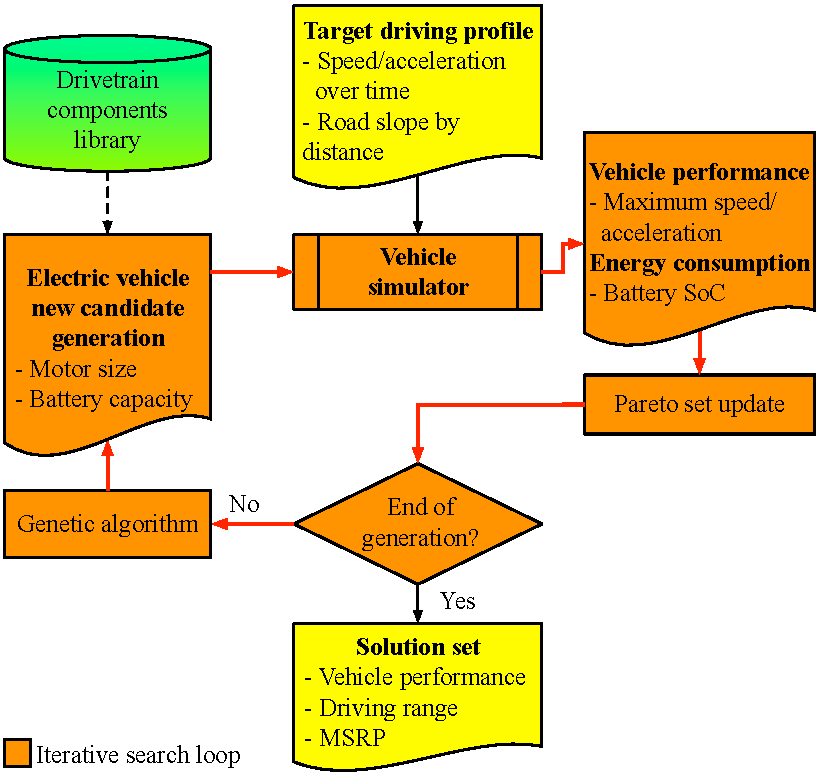
\includegraphics[width=1.0\hsize]{Figures/Naehyuck_Chang/design_optimization.pdf}
\caption{Design-time propulsion power optimization dedicated to a driving mission.}
\label{fig:design_opt}
\end{figure} 


It would be a more proactive energy saving if the energy optimality is considered at design time. Determination of the battery capacity is a really critical factor in electric vehicle unlike internal combustion engine vehicles questioning the gas tank size. The battery capacity directly impacts on the vehicle weight as well as the driving range, vehicle price and space utilization. As observed in Sections~\ref{subsec:propulsion_model} and \ref{subsec:propulsion_runtime_opt}, vehicle weight is a major variables that determines energy efficiency. Installation of a larger-capacity battery certainly increases the driving range but certainly decreases fuel efficiency (MPGe, mile per gallon gasoline equivalent.) Electric vehicles would better not carry an unnecessarily big battery pack while commuting in a short distance. A heavier battery pack also degrades the performance of the electric vehicles. On the other hand, a large capacity battery pack provides clear benefits such as a larger C rating (the Ah of the battery pack) that makes the battery efficiency higher, a lower battery temperature rise and a longer cyclelife. As a result, determination of the battery pack capacity must consider various aspects. To make a long story short, tailored specification of an electric vehicle dedicated to a particular operating scenario gives a huge opportunity to save energy consumption.

Design-time optimization requires extensive evaluation of the vehicle characteristics whenever a design variable is changed. It is not feasible to perform actual driving test during the design time. Automotive original equipment manufacturer (OEM) have been collecting range of data over decades and attempt to find a better empirical setup. Simulation environment can significantly reduces the design effort. Driving energy simulators evaluate the power consumption by changing the powertrain specification and estimate the vehicle performance and driving range as shown in Fig.~\ref{fig:design_opt}. A vehicle simulator on a Matlab evaluates energy consumption by the motor, battery characteristics, gearbox, vehicle chassis, and so on~\cite{Butler:TVT99,Markel:JPS02}. Related previous work optimizes the battery pack capacity for a given driving mission~\cite{Gao:TIE10}. A supercapacitor and battery hybrid can prolong the battery lifetime~\cite{Song:AE14}. The optimal reduction ratio of the traction motor to the wheels also increases the electric vehicle fuel efficiency~\cite{Yin:ITEC-AP14}. Power rating of the traction motor, gear reduction ratio and the battery capacity should be jointly optimized. However, such design space is very big, and evaluation time complexity is huge. Genetic algorithm is a common way to solve such multi-objective optimization, and related work analyzes vehicle efficiency by the motor power rating and the battery capacity~\cite{Pozo:AMAA15}. The design space becomes limited if the available components are in the limited number of libraries. Related work derives the optimal hybrid electric bus with 19 choices of diesel engine power rating, 19 choices of alternator capacities, 28 different size of traction motors, nine battery pack capacity variations, and seven gearbox reduction ratios~\cite{Hasanzadeh:INDEL14}. Similar work attempts the best configuration of passenger vehicles and pickup trucks by the driving scenarios with four fuel cells, four motor power ratings, and eight battery pack capacities using Genetic algorithm~\cite{Ribau:AE14}.


